%%%%%%%%%%%%%%%%%%%%%%%%%%%%%%%%%%%%
% Header                           %
%%%%%%%%%%%%%%%%%%%%%%%%%%%%%%%%%%%%
% 
% Revisions: 2017-04-10 Martin R�del <martin.raedel@dlr.de>
%                       Initial draft
%               
% Contact:   Martin R�del,  martin.raedel@dlr.de
%            DLR Composite Structures and Adaptive Systems
%          
%                                 __/|__
%                                /_/_/_/  
%            www.dlr.de/fa/en      |/ DLR
%
%%%%%%%%%%%%%%%%%%%%%%%%%%%%%%%%%%%%
% Content                          %
%%%%%%%%%%%%%%%%%%%%%%%%%%%%%%%%%%%%

\leveldown{Plot selection data over time}

To plot selection data, e.g. point results, over calculation time perform the following steps:

\begin{enumerate}[noitemsep]
\item Import result file to \marktool{\paraviewname}
\item Create a selection, e.g. to a single or two points
\item From the menu bar:
  \begin{itemize}[noitemsep]
  \item Click Filters
  \item Click Data Analysis
  \item Click \textit{Plot Selection Over Time}
  \end{itemize}
  or click 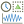
\includegraphics[width=\iconsize]{Figures/Icons/pqPlotSelectionOverTime24} in the Data Analysis toolbar
\item In the newly opened Properties tab:
  \begin{itemize}[noitemsep]
  \item Review the Copied Selection
  \item Click \textit{Apply}
  \item Let \marktool{\paraviewname} process your request a couple of seconds
  \item For the actual values deselect the \textit{Only Report Selection Statistics} checkbox
  \item Click \textit{Apply}
  \item Wait until the progressbar in the bottom right is completed
  \item Select from the selection entities the items you are currently interested in
  \item Choose the \textit{Series Parameters} you are interested in (there is the same quantity for each selection entity, so a couple of times if you have multiple entities in your selection, choose wisely)
  \item Your requested values should show up in the \textit{QuartileChartView}
  \end{itemize}
\item You can skip through the time steps of your analysis in the Current Time Controls toolbar. The current time is shown as the vertical bar in the chart view
\end{enumerate}

To see the actual values in a spreadsheet:

\begin{enumerate}[noitemsep]
\item Right-click on the QuartileChartView top line (where e.g. QuartileChartView1 stands)
\item Create a selection, e.g. to a single or two points
\item Select:
  \begin{itemize}[noitemsep]
  \item Convert To ...
  \item Spreadsheet view
  \end{itemize}
\item In case you want to return to the Chart View you can do so accordingly but you have to repeat the data selection steps mentioned above
\end{enumerate}

A combined view:

\begin{figure}[htbp]
\centering
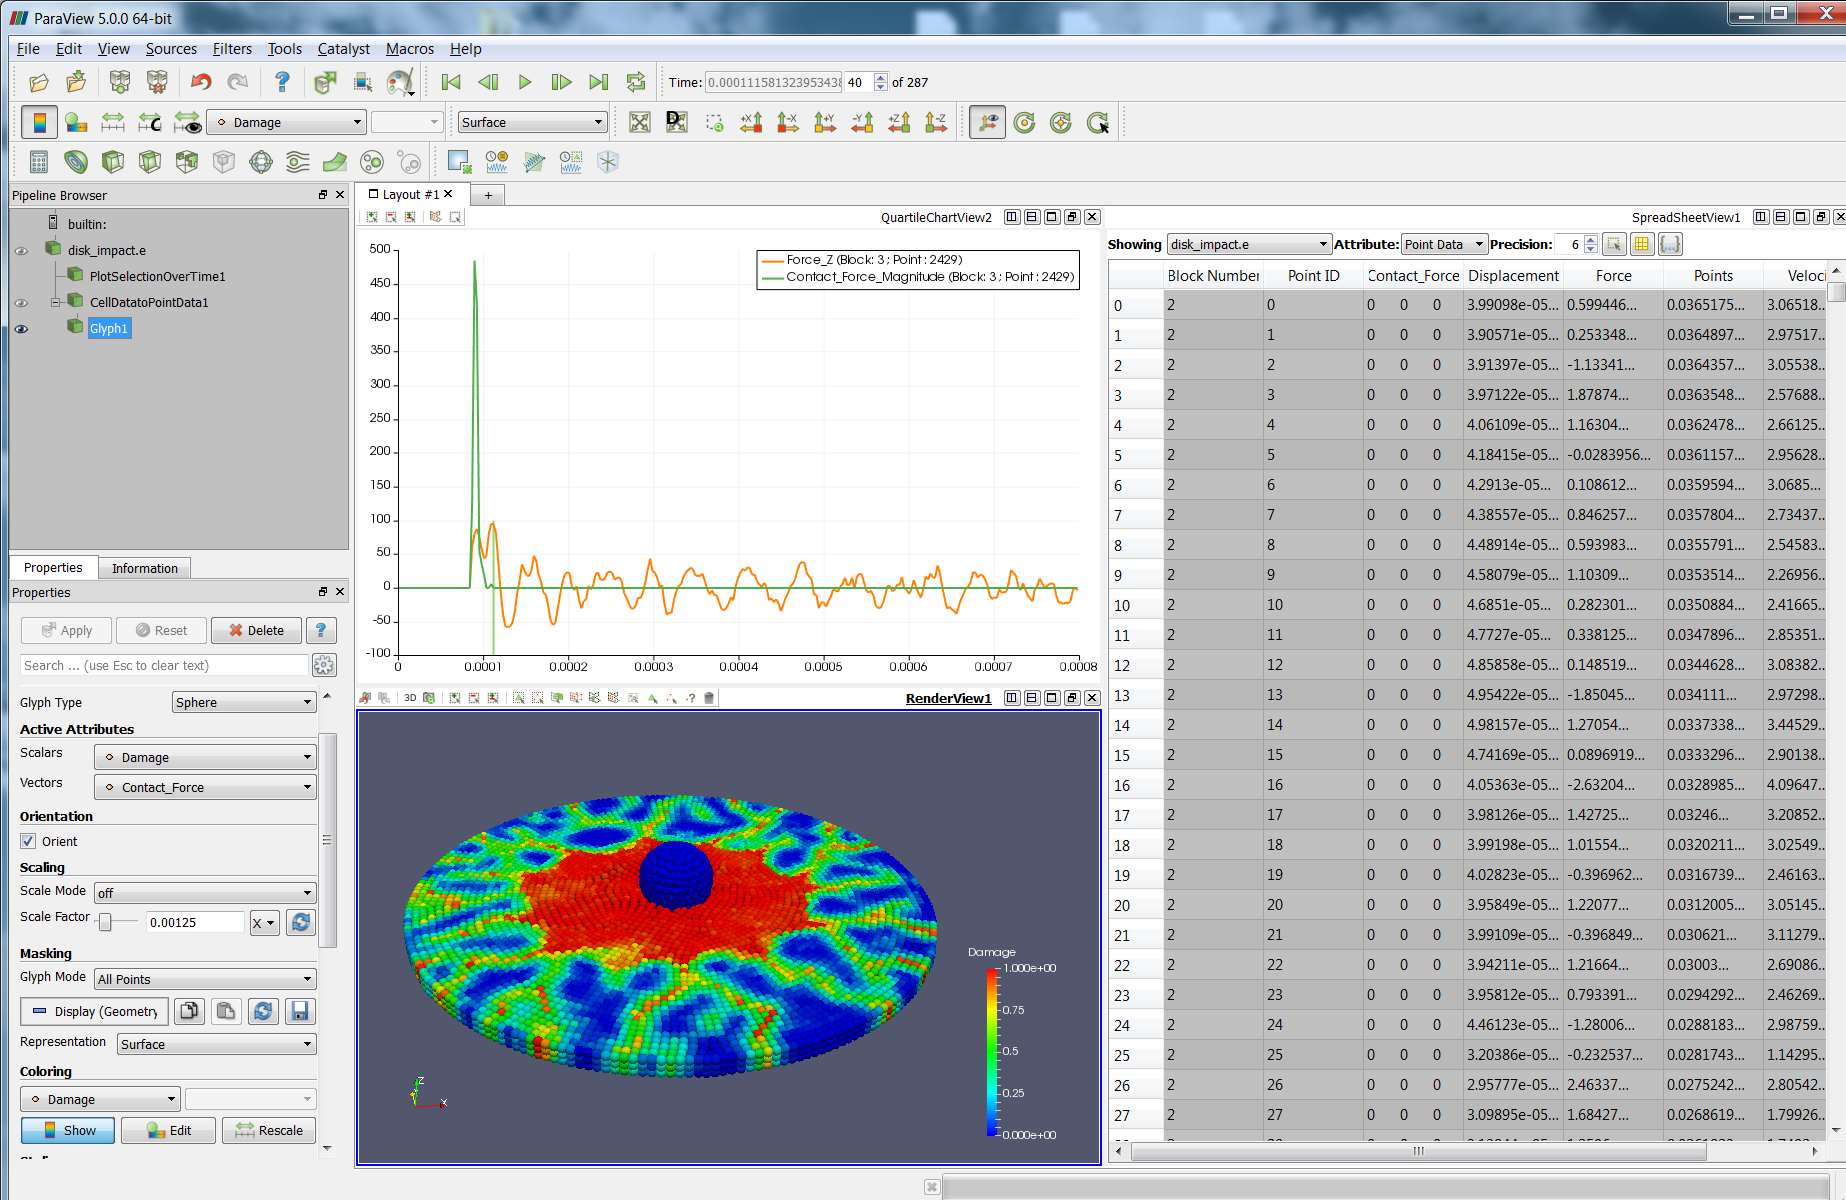
\includegraphics[width=\paraviewscreenshotwidthfac\linewidth]{Figures/Screenshots/State_ChartView_Combined}
\caption{Combined \marktool{\paraviewname} view}
\label{fig:Combined_ParaView_view}
\end{figure}

To save the data for plotting in \verb+pgfplots+:

\begin{enumerate}[noitemsep]
\item Select the PlotOverSelection in the \textit{Pipeline Browser} or left click in the ChartView or SpreadsheetView
\item From the menu bar:
  \begin{itemize}[noitemsep]
  \item Click File
  \item Click Save Data
  \end{itemize}
  or click 
\includegraphics[width=\iconsize]{Figures/Icons/pqSave32} in the Main Controls toolbar
\item Select folder and filename
\item Select csv file type
\item Click \textit{Ok}
\end{enumerate}

Beware, an individual csv-file is written for each and every entity in your selection. The file does not include any information on the entity ID or name. Thus, a sequential save-process for each single individual entity is advised. After each save, rename the resulting file.